\documentclass[]{article}
\usepackage[left=1in,top=1in,right=1in,bottom=1in]{geometry}


%%%% more monte %%%%
% thispagestyle{empty}
% https://stackoverflow.com/questions/2166557/how-to-hide-the-page-number-in-latex-on-first-page-of-a-chapter
\usepackage{color}
\usepackage[table]{xcolor} % are they using color?

\definecolor{WSU.crimson}{HTML}{981e32}
\definecolor{WSU.gray}{HTML}{5e6a71}

\definecolor{shadecolor}{RGB}{248,248,248}
\definecolor{WSU.crimson}{RGB}{152,30,50} % use http://colors.mshaffer.com to convert from 981e32
\definecolor{WSU.gray}{RGB}{94,106,113}

%%%%%%%%%%%%%%%%%%%%%%%%%%%%

\newcommand*{\authorfont}{\fontfamily{phv}\selectfont}
\usepackage{lmodern}


\usepackage[T1]{fontenc}
  \usepackage[utf8]{inputenc}




\usepackage{abstract}
\renewcommand{\abstractname}{}    % clear the title
\renewcommand{\absnamepos}{empty} % originally center

\renewenvironment{abstract}
 {{%
    \setlength{\leftmargin}{0mm}
    \setlength{\rightmargin}{\leftmargin}%
  }%
  \relax}
 {\endlist}

\makeatletter
\def\@maketitle{%
  \pagestyle{empty}
  \newpage
%  \null
%  \vskip 2em%
%  \begin{center}%
  \let \footnote \thanks
    {\fontsize{18}{20}\selectfont\raggedright  \setlength{\parindent}{0pt} \@title \par}%
}
%\fi
\makeatother






\usepackage{color}
\usepackage{fancyvrb}
\newcommand{\VerbBar}{|}
\newcommand{\VERB}{\Verb[commandchars=\\\{\}]}
\DefineVerbatimEnvironment{Highlighting}{Verbatim}{commandchars=\\\{\}}
% Add ',fontsize=\small' for more characters per line
\usepackage{framed}
\definecolor{shadecolor}{RGB}{248,248,248}
\newenvironment{Shaded}{\begin{snugshade}}{\end{snugshade}}
\newcommand{\AlertTok}[1]{\textcolor[rgb]{0.94,0.16,0.16}{#1}}
\newcommand{\AnnotationTok}[1]{\textcolor[rgb]{0.56,0.35,0.01}{\textbf{\textit{#1}}}}
\newcommand{\AttributeTok}[1]{\textcolor[rgb]{0.77,0.63,0.00}{#1}}
\newcommand{\BaseNTok}[1]{\textcolor[rgb]{0.00,0.00,0.81}{#1}}
\newcommand{\BuiltInTok}[1]{#1}
\newcommand{\CharTok}[1]{\textcolor[rgb]{0.31,0.60,0.02}{#1}}
\newcommand{\CommentTok}[1]{\textcolor[rgb]{0.56,0.35,0.01}{\textit{#1}}}
\newcommand{\CommentVarTok}[1]{\textcolor[rgb]{0.56,0.35,0.01}{\textbf{\textit{#1}}}}
\newcommand{\ConstantTok}[1]{\textcolor[rgb]{0.00,0.00,0.00}{#1}}
\newcommand{\ControlFlowTok}[1]{\textcolor[rgb]{0.13,0.29,0.53}{\textbf{#1}}}
\newcommand{\DataTypeTok}[1]{\textcolor[rgb]{0.13,0.29,0.53}{#1}}
\newcommand{\DecValTok}[1]{\textcolor[rgb]{0.00,0.00,0.81}{#1}}
\newcommand{\DocumentationTok}[1]{\textcolor[rgb]{0.56,0.35,0.01}{\textbf{\textit{#1}}}}
\newcommand{\ErrorTok}[1]{\textcolor[rgb]{0.64,0.00,0.00}{\textbf{#1}}}
\newcommand{\ExtensionTok}[1]{#1}
\newcommand{\FloatTok}[1]{\textcolor[rgb]{0.00,0.00,0.81}{#1}}
\newcommand{\FunctionTok}[1]{\textcolor[rgb]{0.00,0.00,0.00}{#1}}
\newcommand{\ImportTok}[1]{#1}
\newcommand{\InformationTok}[1]{\textcolor[rgb]{0.56,0.35,0.01}{\textbf{\textit{#1}}}}
\newcommand{\KeywordTok}[1]{\textcolor[rgb]{0.13,0.29,0.53}{\textbf{#1}}}
\newcommand{\NormalTok}[1]{#1}
\newcommand{\OperatorTok}[1]{\textcolor[rgb]{0.81,0.36,0.00}{\textbf{#1}}}
\newcommand{\OtherTok}[1]{\textcolor[rgb]{0.56,0.35,0.01}{#1}}
\newcommand{\PreprocessorTok}[1]{\textcolor[rgb]{0.56,0.35,0.01}{\textit{#1}}}
\newcommand{\RegionMarkerTok}[1]{#1}
\newcommand{\SpecialCharTok}[1]{\textcolor[rgb]{0.00,0.00,0.00}{#1}}
\newcommand{\SpecialStringTok}[1]{\textcolor[rgb]{0.31,0.60,0.02}{#1}}
\newcommand{\StringTok}[1]{\textcolor[rgb]{0.31,0.60,0.02}{#1}}
\newcommand{\VariableTok}[1]{\textcolor[rgb]{0.00,0.00,0.00}{#1}}
\newcommand{\VerbatimStringTok}[1]{\textcolor[rgb]{0.31,0.60,0.02}{#1}}
\newcommand{\WarningTok}[1]{\textcolor[rgb]{0.56,0.35,0.01}{\textbf{\textit{#1}}}}

\usepackage{graphicx,grffile}
\makeatletter
\def\maxwidth{\ifdim\Gin@nat@width>\linewidth\linewidth\else\Gin@nat@width\fi}
\def\maxheight{\ifdim\Gin@nat@height>\textheight\textheight\else\Gin@nat@height\fi}
\makeatother
% Scale images if necessary, so that they will not overflow the page
% margins by default, and it is still possible to overwrite the defaults
% using explicit options in \includegraphics[width, height, ...]{}
\setkeys{Gin}{width=\maxwidth,height=\maxheight,keepaspectratio}


\title{\textbf{\textcolor{WSU.crimson}{Will V. Denzel}}  }
 

%  

% \author{ \Large true \hfill \normalsize \emph{} }
\author{\Large Joshua
Bennett\vspace{0.05in} \newline\normalsize\emph{Washington State
University}  }


\date{December 14, 2020}
\setcounter{secnumdepth}{3}

\usepackage{titlesec}
% See the link above: KOMA classes are not compatible with titlesec any more. Sorry.
% https://github.com/jbezos/titlesec/issues/11
\titleformat*{\section}{\bfseries}
\titleformat*{\subsection}{\bfseries\itshape}
\titleformat*{\subsubsection}{\itshape}
\titleformat*{\paragraph}{\itshape}
\titleformat*{\subparagraph}{\itshape}

% https://code.usgs.gov/usgs/norock/irvine_k/ip-092225/


%\titleformat*{\section}{\normalsize\bfseries}
%\titleformat*{\subsection}{\normalsize\itshape}
%\titleformat*{\subsubsection}{\normalsize\itshape}
%\titleformat*{\paragraph}{\normalsize\itshape}
%\titleformat*{\subparagraph}{\normalsize\itshape}

% https://tex.stackexchange.com/questions/233866/one-column-multicol-environment#233904
\usepackage{environ}
\NewEnviron{auxmulticols}[1]{%
  \ifnum#1<2\relax% Fewer than 2 columns
    %\vspace{-\baselineskip}% Possible vertical correction
    \BODY
  \else% More than 1 column
    \begin{multicols}{#1}
      \BODY
    \end{multicols}%
  \fi
}





\usepackage{natbib}
\setcitestyle{aysep={}} %% no year, comma just year
% \usepackage[numbers]{natbib}
\bibliographystyle{./../biblio/ormsv080.bst}



\usepackage[strings]{underscore} % protect underscores in most circumstances




\newtheorem{hypothesis}{Hypothesis}
\usepackage{setspace}


%%%%%%%%%%%%%%%%%%%%%%%%%%%%%%%%%%%%%%%%%%%%%%%%%%%%%
%%% MONTE ADDS %%%

\usepackage{fancyhdr} % fancy header 
\usepackage{lastpage} % last page 

\usepackage{multicol}


\usepackage{etoolbox}
\AtBeginEnvironment{quote}{\singlespacing\small}
% https://tex.stackexchange.com/questions/325695/how-to-style-blockquote


\usepackage{soul}			%% allows strike-through
\usepackage{url}			%% fixes underscores in urls
\usepackage{csquotes}		%% allows \textquote in references
\usepackage{rotating}		%% allows table and box rotation
\usepackage{caption}		%% customize caption information
\usepackage{booktabs}		%% enhance table/tabular environment
\usepackage{tabularx}		%% width attributes updates tabular
\usepackage{enumerate}		%% special item environment
\usepackage{enumitem}		%% special item environment

\usepackage{lineno}		%% allows linenumbers for editing using \linenumbers
\usepackage{hanging}


\usepackage{mathtools}  	%% also loads amsmath
\usepackage{bm}		%% bold-math
\usepackage{scalerel}	%% scale one element (make one beta bigger font)

\newcommand{\gFrac}[2]{ \genfrac{}{}{0pt}{1}{{#1}}{#2} }

\newcommand{\betaSH}[3]{  \gFrac{\text{\tiny #1}}{{\text{\tiny #2}}}\hat{\beta}_{\text{#3}}   }
\newcommand{\betaSB}[3]{              ^{\text{#1}} _{\text{#2}} \bm{\beta} _{\text{#3}}                   }  %% bold
\newcommand{\bigEQ}{  \scaleobj{1.5}{{\ }= } }
\newcommand{\bigP}[1]{  \scaleobj{1.5}{#1 } }





\usepackage{endnotes}  % he already does this ...
\renewcommand{\enotesize}{\normalsize}
% https://tex.stackexchange.com/questions/99984/endnotes-do-not-be-superscript-and-add-a-space
\renewcommand\makeenmark{\textsuperscript{[\theenmark]}} % in brackets %
% https://tex.stackexchange.com/questions/31574/how-to-control-the-indent-in-endnotes
\patchcmd{\enoteformat}{1.8em}{0pt}{}{}

\patchcmd{\theendnotes}
  {\makeatletter}
  {\makeatletter\renewcommand\makeenmark{\textbf{[\theenmark]} }}
  {}{}



% https://tex.stackexchange.com/questions/141906/configuring-footnote-position-and-spacing

\addtolength{\footnotesep}{5mm} % change to 1mm

\renewcommand{\thefootnote}{\textbf{\arabic{footnote}}}
\let\footnote=\endnote
%\renewcommand*{\theendnote}{\alph{endnote}}
%\renewcommand{\theendnote}{\textbf{\arabic{endnote}}}


\renewcommand*{\notesname}{ENDNOTES}

\makeatletter
\def\enoteheading{\section*{\notesname
  \@mkboth{\MakeUppercase{\notesname}}{\MakeUppercase{\notesname}}}%
  \mbox{}\par\vskip-2.3\baselineskip\noindent\rule{.5\textwidth}{0.4pt}\par\vskip\baselineskip}
\makeatother


\renewcommand*{\contentsname}{TABLE OF CONTENTS}

\renewcommand*{\refname}{REFERENCES}


%\usepackage{subfigure}
\usepackage{subcaption}

\captionsetup{labelfont=bf}  % Make Table / Figure bold

%%% you could add elements here ... monte says .... %%%
%\usepackage{mypackageForCapitalH}


%%%%%%%%%%%%%%%%%%%%%%%%%%%%%%%%%%%%%%%%%%%%%%%%%%%%%

% set default figure placement to htbp
\makeatletter
\def\fps@figure{htbp}
\makeatother


% move the hyperref stuff down here, after header-includes, to allow for - \usepackage{hyperref}

\makeatletter
\@ifpackageloaded{hyperref}{}{%
\ifxetex
  \PassOptionsToPackage{hyphens}{url}\usepackage[setpagesize=false, % page size defined by xetex
              unicode=false, % unicode breaks when used with xetex
              xetex]{hyperref}
\else
  \PassOptionsToPackage{hyphens}{url}\usepackage[draft,unicode=true]{hyperref}
\fi
}

\@ifpackageloaded{color}{
    \PassOptionsToPackage{usenames,dvipsnames}{color}
}{%
    \usepackage[usenames,dvipsnames]{color}
}
\makeatother
\hypersetup{breaklinks=true,
            bookmarks=true,
            pdfauthor={Joshua Bennett (Washington State University)},
             pdfkeywords = {T-tests, Histogram, Data Integrity,
ScatterPlot, correlation tables},  
            pdftitle={Will V. Denzel},
            colorlinks=true,
            citecolor=blue,
            urlcolor=blue,
            linkcolor=magenta,
            pdfborder={0 0 0}}
\urlstyle{same}  % don't use monospace font for urls

% Add an option for endnotes. -----

%
% add tightlist ----------
\providecommand{\tightlist}{%
\setlength{\itemsep}{0pt}\setlength{\parskip}{0pt}}

% add some other packages ----------

% \usepackage{multicol}
% This should regulate where figures float
% See: https://tex.stackexchange.com/questions/2275/keeping-tables-figures-close-to-where-they-are-mentioned
\usepackage[section]{placeins}



\pagestyle{fancy}   
\lhead{\textcolor{WSU.crimson}{\textbf{ Will V. Denzel }}}
\chead{}
\rhead{\textcolor{WSU.gray}{\textbf{  Page\ \thepage\ of\ \protect\pageref{LastPage} }}}
\lfoot{}
\cfoot{}
\rfoot{}


\begin{document}
	
% \pagenumbering{arabic}% resets `page` counter to 1 
%    

% \maketitle

{% \usefont{T1}{pnc}{m}{n}
\setlength{\parindent}{0pt}
\thispagestyle{plain}
{\fontsize{18}{20}\selectfont\raggedright 
\maketitle  % title \par  

}

{
   \vskip 13.5pt\relax \normalsize\fontsize{11}{12} 
   
\textbf{\authorfont Joshua Bennett} \hskip 15pt \emph{\small Washington
State University}   

}

}








\begin{abstract}

    \hbox{\vrule height .2pt width 39.14pc}

    \vskip 8.5pt % \small 

\noindent In this Article we will discuss who is the better artor
between Will Smith and Denzel Washington.


\vskip 8.5pt \noindent \textbf{\underline{Keywords}:} T-tests,
Histogram, Data Integrity, ScatterPlot, correlation tables \par

    




    
    \hbox{\vrule height .2pt width 39.14pc}
    \vskip 5pt 
    \hfill \textbf{\textcolor{WSU.gray}{ December 14, 2020 } }
    \vskip 5pt 
    
\end{abstract}


\vskip -8.5pt



 % removetitleabstract

\noindent  

\begin{Shaded}
\begin{Highlighting}[]
\KeywordTok{library}\NormalTok{(devtools);}
\end{Highlighting}
\end{Shaded}

\begin{verbatim}
## Loading required package: usethis
\end{verbatim}

\begin{Shaded}
\begin{Highlighting}[]
\KeywordTok{library}\NormalTok{(humanVerseWSU);}

\NormalTok{path.github =}\StringTok{ "https://raw.githubusercontent.com/MonteShaffer/humanVerseWSU/master/"}\NormalTok{;}

\NormalTok{include.me =}\StringTok{ }\KeywordTok{paste0}\NormalTok{(path.github, }\StringTok{"misc/functions{-}nlp.R"}\NormalTok{);}
\KeywordTok{source\_url}\NormalTok{( include.me );}
\end{Highlighting}
\end{Shaded}

\begin{verbatim}
## SHA-1 hash of file is 704afa69d52215d315cb5f59cdc020b0bbfd0b13
\end{verbatim}

\begin{verbatim}
## Warning: package 'tm' was built under R version 4.0.3
\end{verbatim}

\begin{verbatim}
## Loading required package: NLP
\end{verbatim}

\begin{verbatim}
## Warning: package 'NLP' was built under R version 4.0.3
\end{verbatim}

\begin{verbatim}
## Warning: package 'SentimentAnalysis' was built under R version 4.0.3
\end{verbatim}

\begin{verbatim}
## 
## Attaching package: 'SentimentAnalysis'
\end{verbatim}

\begin{verbatim}
## The following object is masked from 'package:base':
## 
##     write
\end{verbatim}

\begin{Shaded}
\begin{Highlighting}[]
\NormalTok{include.me =}\StringTok{ }\KeywordTok{paste0}\NormalTok{(path.github, }\StringTok{"misc/functions{-}nlp{-}str.R"}\NormalTok{);}
\KeywordTok{source\_url}\NormalTok{( include.me );}
\end{Highlighting}
\end{Shaded}

\begin{verbatim}
## SHA-1 hash of file is 6bdb234fa84eea995969dc29d6ff2a78f3982131
\end{verbatim}

\begin{Shaded}
\begin{Highlighting}[]
\NormalTok{include.me =}\StringTok{ }\KeywordTok{paste0}\NormalTok{(path.github, }\StringTok{"misc/functions{-}nlp{-}stack.R"}\NormalTok{);}
\KeywordTok{source\_url}\NormalTok{( include.me );}
\end{Highlighting}
\end{Shaded}

\begin{verbatim}
## SHA-1 hash of file is 034efbce0405954198545f8798e119b77a4809c9
\end{verbatim}

\begin{Shaded}
\begin{Highlighting}[]
\NormalTok{include.me =}\StringTok{ }\KeywordTok{paste0}\NormalTok{(path.github, }\StringTok{"misc/functions{-}nlp{-}pos.R"}\NormalTok{);}
\KeywordTok{source\_url}\NormalTok{( include.me );}
\end{Highlighting}
\end{Shaded}

\begin{verbatim}
## SHA-1 hash of file is d8c8cf01c8ead1b6d4228891aa52bac77084a6e7
\end{verbatim}

\begin{verbatim}
## Warning: package 'openNLP' was built under R version 4.0.3
\end{verbatim}

\begin{Shaded}
\begin{Highlighting}[]
\NormalTok{include.me =}\StringTok{ }\KeywordTok{paste0}\NormalTok{(path.github, }\StringTok{"humanVerseWSU/R/functions{-}encryption.R"}\NormalTok{);}
\KeywordTok{source\_url}\NormalTok{( include.me );}
\end{Highlighting}
\end{Shaded}

\begin{verbatim}
## SHA-1 hash of file is da71dde620bed33db055778b752eefb476f7bf6b
\end{verbatim}

\begin{Shaded}
\begin{Highlighting}[]
\NormalTok{include.me =}\StringTok{ }\KeywordTok{paste0}\NormalTok{(path.github,}\StringTok{"misc/functions{-}project{-}measure.R"}\NormalTok{);}
\KeywordTok{source\_url}\NormalTok{( include.me);}
\end{Highlighting}
\end{Shaded}

\begin{verbatim}
## SHA-1 hash of file is 091aa1c443f262dce181395047d037a756331a65
\end{verbatim}

\begin{verbatim}
## Warning: package 'Hmisc' was built under R version 4.0.3
\end{verbatim}

\begin{verbatim}
## Loading required package: lattice
\end{verbatim}

\begin{verbatim}
## Loading required package: survival
\end{verbatim}

\begin{verbatim}
## Loading required package: Formula
\end{verbatim}

\begin{verbatim}
## Loading required package: ggplot2
\end{verbatim}

\begin{verbatim}
## 
## Attaching package: 'ggplot2'
\end{verbatim}

\begin{verbatim}
## The following object is masked from 'package:NLP':
## 
##     annotate
\end{verbatim}

\begin{verbatim}
## 
## Attaching package: 'Hmisc'
\end{verbatim}

\begin{verbatim}
## The following objects are masked from 'package:base':
## 
##     format.pval, units
\end{verbatim}

\begin{Shaded}
\begin{Highlighting}[]
\NormalTok{path.to.nascent =}\StringTok{ "C:/Users/Alexander Nevsky/Dropbox/WSU{-}419/Fall 2020/\_\_student\_access\_\_/unit\_02\_confirmatory\_data\_analysis/nascent/"}\NormalTok{;}

\NormalTok{folder.nlp =}\StringTok{ "nlp/"}\NormalTok{;}
\NormalTok{path.to.nlp =}\StringTok{ }\KeywordTok{paste0}\NormalTok{(path.to.nascent, folder.nlp);}


\CommentTok{\#\#\#\#\#\# UPDATES TO dataframe subset function \#\#\#\#\#\#}
\CommentTok{\# inflation adjustments for NA ... and improvements on subsetting}
\NormalTok{include.me =}\StringTok{ }\KeywordTok{paste0}\NormalTok{(path.github, }\StringTok{"humanVerseWSU/R/functions{-}dataframe.R"}\NormalTok{);}
\KeywordTok{source\_url}\NormalTok{( include.me );}
\end{Highlighting}
\end{Shaded}

\begin{verbatim}
## SHA-1 hash of file is 1149cbf3e865f692b50d4d1983e6364dc56ce62d
\end{verbatim}

\begin{Shaded}
\begin{Highlighting}[]
\NormalTok{include.me =}\StringTok{ }\KeywordTok{paste0}\NormalTok{(path.github, }\StringTok{"humanVerseWSU/R/functions{-}inflation.R"}\NormalTok{);}
\KeywordTok{source\_url}\NormalTok{( include.me );}
\end{Highlighting}
\end{Shaded}

\begin{verbatim}
## SHA-1 hash of file is b6d29327e3fe030ca132b135f4a89b6fc6a61a66
\end{verbatim}

\hypertarget{imdb-custom-library}{%
\section{(IMDB) Custom library}\label{imdb-custom-library}}

This is a large dataset I harvested in September. It will allow us to
explore more comprehensively the relationships of various features of
the movie database. It is large (about 50MB), so installing may take
some time if you are on a slow internet connection.

This dataset will be the source you will use on your final exam to
answer the question posed earlier in the semester about Will Smith and
Denzel Washington. You now have more analytics skills and with the new
dataset there are more features you can extract.

\begin{Shaded}
\begin{Highlighting}[]
\CommentTok{\# library(devtools);}
\CommentTok{\# install\_github("MonteShaffer/imdb/imdb"); \# choose \#3 to humanVerseWSU}
\CommentTok{\# detach(package:imdb);}
\KeywordTok{library}\NormalTok{(imdb);}
\KeywordTok{packageVersion}\NormalTok{(}\StringTok{"imdb"}\NormalTok{);  }\CommentTok{\# ‘0.1.1’}
\end{Highlighting}
\end{Shaded}

\begin{verbatim}
## [1] '0.1.1'
\end{verbatim}

\begin{Shaded}
\begin{Highlighting}[]
\CommentTok{\# ?loadDataIMDB}
\end{Highlighting}
\end{Shaded}

\hypertarget{load-data}{%
\subsection{Load data}\label{load-data}}

Once this is run, a lot of memory will be required to read in the 23
compressed files.

\begin{Shaded}
\begin{Highlighting}[]
\KeywordTok{install\_github}\NormalTok{(}\StringTok{"MonteShaffer/imdb/imdb"}\NormalTok{)}
\end{Highlighting}
\end{Shaded}

\begin{verbatim}
## Skipping install of 'imdb' from a github remote, the SHA1 (b29c6691) has not changed since last install.
##   Use `force = TRUE` to force installation
\end{verbatim}

\begin{Shaded}
\begin{Highlighting}[]
\NormalTok{imdb}\OperatorTok{::}\KeywordTok{loadDataIMDB}\NormalTok{();}
\KeywordTok{names}\NormalTok{(imdb.data);}
\end{Highlighting}
\end{Shaded}

\begin{verbatim}
##  [1] "all.movies.creatives"         "all.movies.companies"        
##  [3] "all.movies.actors.characters" "all.actors.rank"             
##  [5] "all.actors.movies"            "all.actors.info"             
##  [7] "moviecount.byyear"            "actors"                      
##  [9] "glue"                         "headliners"                  
## [11] "movies"                       "movies.df"
\end{verbatim}

\begin{Shaded}
\begin{Highlighting}[]
\NormalTok{humanVerseWSU}\OperatorTok{::}\KeywordTok{loadInflationData}\NormalTok{();}
\end{Highlighting}
\end{Shaded}

Create Dataframe for the top gross and best reviews movies

\begin{Shaded}
\begin{Highlighting}[]
\KeywordTok{library}\NormalTok{(KernSmooth)}
\end{Highlighting}
\end{Shaded}

\begin{verbatim}
## Warning: package 'KernSmooth' was built under R version 4.0.3
\end{verbatim}

\begin{verbatim}
## KernSmooth 2.23 loaded
## Copyright M. P. Wand 1997-2009
\end{verbatim}

\begin{Shaded}
\begin{Highlighting}[]
\NormalTok{normalDiagnosticPlot =}\StringTok{ }\ControlFlowTok{function}\NormalTok{(x,  }\DataTypeTok{normalityTest=}\OtherTok{TRUE}\NormalTok{,}
                                    \DataTypeTok{showDensity=}\OtherTok{TRUE}\NormalTok{,}
                                    \DataTypeTok{showNormal=}\OtherTok{TRUE}\NormalTok{,}
                                    \DataTypeTok{showSDs=}\OtherTok{FALSE}\NormalTok{,}
                                    \DataTypeTok{showAxis=}\OtherTok{TRUE}
\NormalTok{                                )}
\NormalTok{  \{}
\NormalTok{  xx =}\StringTok{ }\KeywordTok{na.omit}\NormalTok{(x);}
\NormalTok{  x.stats =}\StringTok{ }\KeywordTok{doStatsSummary}\NormalTok{(x);}
  \CommentTok{\# x.table = table(x);}
  
  \CommentTok{\# library(KernSmooth); \# install.packages("KernSmooth", dependencies=TRUE);}
  \CommentTok{\# bin.count = dpih(xx);}
  \CommentTok{\# mybreaks = 100 * bin.count;}
  
\NormalTok{  mxlim =}\StringTok{ }\KeywordTok{c}\NormalTok{(x.stats}\OperatorTok{$}\NormalTok{mean }\OperatorTok{{-}}\StringTok{ }\FloatTok{3.5} \OperatorTok{*}\StringTok{ }\NormalTok{x.stats}\OperatorTok{$}\NormalTok{sd , }
\NormalTok{            x.stats}\OperatorTok{$}\NormalTok{mean }\OperatorTok{+}\StringTok{ }\FloatTok{3.5} \OperatorTok{*}\StringTok{ }\NormalTok{x.stats}\OperatorTok{$}\NormalTok{sd );}
\NormalTok{  h =}\StringTok{ }\KeywordTok{hist}\NormalTok{(xx, }\DataTypeTok{breaks=}\StringTok{"Sturges"}\NormalTok{, }\DataTypeTok{plot=}\NormalTok{F);}
\NormalTok{  mylim =}\StringTok{ }\KeywordTok{c}\NormalTok{(}\DecValTok{0}\NormalTok{, }\KeywordTok{max}\NormalTok{(h}\OperatorTok{$}\NormalTok{counts));}
  
\NormalTok{  myMain =}\StringTok{ }\KeywordTok{paste0}\NormalTok{(  }\StringTok{"Histogram (mean: "}\NormalTok{,}
                  \KeywordTok{round}\NormalTok{(x.stats}\OperatorTok{$}\NormalTok{mean,}\DataTypeTok{digits=}\DecValTok{3}\NormalTok{), }
                  \StringTok{", sd: "}\NormalTok{,}
                  \KeywordTok{round}\NormalTok{(x.stats}\OperatorTok{$}\NormalTok{sd,}\DataTypeTok{digits=}\DecValTok{3}\NormalTok{),}
                  \StringTok{")"}
\NormalTok{                  );}
  
  
  
\NormalTok{mxlab =}\StringTok{ ""}\NormalTok{;  }
  \ControlFlowTok{if}\NormalTok{(normalityTest)}
\NormalTok{    \{}
\NormalTok{    isNormal =}\StringTok{ }\OtherTok{NULL}\NormalTok{;}
    \ControlFlowTok{if}\NormalTok{(x.stats}\OperatorTok{$}\NormalTok{shapiro.is.normal}\OperatorTok{$}\StringTok{\textasciigrave{}}\DataTypeTok{0.10}\StringTok{\textasciigrave{}}\NormalTok{) \{ isNormal =}\StringTok{ }\FloatTok{0.10}\NormalTok{; \}}
    \ControlFlowTok{if}\NormalTok{(x.stats}\OperatorTok{$}\NormalTok{shapiro.is.normal}\OperatorTok{$}\StringTok{\textasciigrave{}}\DataTypeTok{0.05}\StringTok{\textasciigrave{}}\NormalTok{) \{ isNormal =}\StringTok{ }\FloatTok{0.05}\NormalTok{; \}}
    \ControlFlowTok{if}\NormalTok{(x.stats}\OperatorTok{$}\NormalTok{shapiro.is.normal}\OperatorTok{$}\StringTok{\textasciigrave{}}\DataTypeTok{0.01}\StringTok{\textasciigrave{}}\NormalTok{) \{ isNormal =}\StringTok{ }\FloatTok{0.01}\NormalTok{; \}}
    
\NormalTok{    isNormalResult =}\StringTok{ }\OtherTok{FALSE}\NormalTok{;}
    \ControlFlowTok{if}\NormalTok{(}\OperatorTok{!}\KeywordTok{is.null}\NormalTok{(isNormal)) \{ isNormalResult =}\StringTok{ }\OtherTok{TRUE}\NormalTok{;\}}
    \ControlFlowTok{if}\NormalTok{(}\KeywordTok{is.null}\NormalTok{(isNormal)) \{ isNormal =}\StringTok{ }\FloatTok{0.05}\NormalTok{;\}}
    
\NormalTok{    mxlab =}\StringTok{ }\KeywordTok{paste0}\NormalTok{(}\StringTok{"Shapiro Normality test at (alpha = "}\NormalTok{,}
\NormalTok{                isNormal, }\StringTok{") is ... "}\NormalTok{,isNormalResult);}
\NormalTok{    \}}
  
  
\CommentTok{\#\#\# Histogram  }
  \KeywordTok{hist}\NormalTok{(xx, }\DataTypeTok{breaks=}\StringTok{"Sturges"}\NormalTok{,  }\DataTypeTok{xlim=}\NormalTok{mxlim, }\DataTypeTok{ylim=}\NormalTok{mylim,}
      \DataTypeTok{xlab=}\NormalTok{mxlab, }\DataTypeTok{xaxt=}\StringTok{\textquotesingle{}n\textquotesingle{}}\NormalTok{, }\DataTypeTok{main=}\NormalTok{myMain);}
  
  \ControlFlowTok{if}\NormalTok{(showDensity)}
\NormalTok{    \{}
    \KeywordTok{par}\NormalTok{(}\DataTypeTok{new=}\NormalTok{T); }\CommentTok{\# overlay}
  \CommentTok{\#\#\# Density Plot (remember first reading?)}
    \KeywordTok{plot}\NormalTok{( }\KeywordTok{density}\NormalTok{(xx, }\DataTypeTok{kernel=}\StringTok{"epanechnikov"}\NormalTok{) ,}
            \DataTypeTok{xlim=}\NormalTok{mxlim, }
            \DataTypeTok{main=}\StringTok{""}\NormalTok{, }
            \DataTypeTok{xlab=}\StringTok{""}\NormalTok{, }
            \DataTypeTok{ylab=}\StringTok{""}\NormalTok{, }
            \DataTypeTok{xaxt=}\StringTok{\textquotesingle{}n\textquotesingle{}}\NormalTok{, }
            \DataTypeTok{yaxt=}\StringTok{\textquotesingle{}n\textquotesingle{}}  
\NormalTok{        );}
\NormalTok{    \}}
    
  
  \ControlFlowTok{if}\NormalTok{(showNormal)}
\NormalTok{    \{    }
    \KeywordTok{par}\NormalTok{(}\DataTypeTok{new=}\NormalTok{T); }\CommentTok{\# overlay  }
  \CommentTok{\#\#\# Normal Curve}
\NormalTok{    xt =}\StringTok{ }\KeywordTok{seq}\NormalTok{(}\OperatorTok{{-}}\FloatTok{3.5}\NormalTok{,}\FloatTok{3.5}\NormalTok{, }\DataTypeTok{length=}\DecValTok{100}\NormalTok{);}
\NormalTok{            yt =}\StringTok{ }\KeywordTok{dnorm}\NormalTok{(xt);}
  
    \KeywordTok{plot}\NormalTok{( xt, yt, }
          \DataTypeTok{type=}\StringTok{"l"}\NormalTok{, }
          \DataTypeTok{lwd=}\DecValTok{2}\NormalTok{, }
          \DataTypeTok{col =} \StringTok{"red"}\NormalTok{,}
          \DataTypeTok{axes=}\NormalTok{F, }
          \DataTypeTok{xlab=}\StringTok{""}\NormalTok{,}
          \DataTypeTok{ylab=}\StringTok{""}
\NormalTok{        );  }
\NormalTok{    \}}
    
    
  \ControlFlowTok{if}\NormalTok{(showSDs)}
\NormalTok{    \{}
  \CommentTok{\#\#\# vertical lines at sd\textquotesingle{}s of data ...    }
    \KeywordTok{abline}\NormalTok{(}\DataTypeTok{v=}\NormalTok{x.stats}\OperatorTok{$}\NormalTok{mean,}\DataTypeTok{lwd=}\DecValTok{4}\NormalTok{,}\DataTypeTok{col=}\StringTok{"blue"}\NormalTok{);}
      \KeywordTok{abline}\NormalTok{(}\DataTypeTok{v=}\NormalTok{x.stats}\OperatorTok{$}\NormalTok{mean }\OperatorTok{{-}}\StringTok{ }\DecValTok{1} \OperatorTok{*}\StringTok{ }\NormalTok{x.stats}\OperatorTok{$}\NormalTok{sd , }\DataTypeTok{col=}\StringTok{"green"}\NormalTok{,}\DataTypeTok{lwd=}\DecValTok{3}\NormalTok{);}
      \KeywordTok{abline}\NormalTok{(}\DataTypeTok{v=}\NormalTok{x.stats}\OperatorTok{$}\NormalTok{mean }\OperatorTok{+}\StringTok{ }\DecValTok{1} \OperatorTok{*}\StringTok{ }\NormalTok{x.stats}\OperatorTok{$}\NormalTok{sd , }\DataTypeTok{col=}\StringTok{"green"}\NormalTok{,}\DataTypeTok{lwd=}\DecValTok{3}\NormalTok{);}
      \KeywordTok{abline}\NormalTok{(}\DataTypeTok{v=}\NormalTok{x.stats}\OperatorTok{$}\NormalTok{mean }\OperatorTok{{-}}\StringTok{ }\DecValTok{2} \OperatorTok{*}\StringTok{ }\NormalTok{x.stats}\OperatorTok{$}\NormalTok{sd , }\DataTypeTok{col=}\StringTok{"green"}\NormalTok{,}\DataTypeTok{lwd=}\DecValTok{2}\NormalTok{);}
      \KeywordTok{abline}\NormalTok{(}\DataTypeTok{v=}\NormalTok{x.stats}\OperatorTok{$}\NormalTok{mean }\OperatorTok{+}\StringTok{ }\DecValTok{2} \OperatorTok{*}\StringTok{ }\NormalTok{x.stats}\OperatorTok{$}\NormalTok{sd , }\DataTypeTok{col=}\StringTok{"green"}\NormalTok{,}\DataTypeTok{lwd=}\DecValTok{2}\NormalTok{);}
      \KeywordTok{abline}\NormalTok{(}\DataTypeTok{v=}\NormalTok{x.stats}\OperatorTok{$}\NormalTok{mean }\OperatorTok{{-}}\StringTok{ }\DecValTok{3} \OperatorTok{*}\StringTok{ }\NormalTok{x.stats}\OperatorTok{$}\NormalTok{sd , }\DataTypeTok{col=}\StringTok{"green"}\NormalTok{,}\DataTypeTok{lwd=}\DecValTok{1}\NormalTok{);}
      \KeywordTok{abline}\NormalTok{(}\DataTypeTok{v=}\NormalTok{x.stats}\OperatorTok{$}\NormalTok{mean }\OperatorTok{+}\StringTok{ }\DecValTok{3} \OperatorTok{*}\StringTok{ }\NormalTok{x.stats}\OperatorTok{$}\NormalTok{sd , }\DataTypeTok{col=}\StringTok{"green"}\NormalTok{,}\DataTypeTok{lwd=}\DecValTok{1}\NormalTok{);}
\NormalTok{    \}}
  
    
  \ControlFlowTok{if}\NormalTok{(showAxis)}
\NormalTok{    \{}
  \CommentTok{\#\#\# axis labels showing the ability to use expression         }
    \KeywordTok{axis}\NormalTok{(}\DecValTok{1}\NormalTok{, }\DataTypeTok{at =} \DecValTok{{-}3}\OperatorTok{:}\DecValTok{3}\NormalTok{, }\DataTypeTok{labels =} \KeywordTok{c}\NormalTok{( }\KeywordTok{expression}\NormalTok{(}\StringTok{"{-}3"}\OperatorTok{\textasciitilde{}}\KeywordTok{hat}\NormalTok{(sigma) ), }\KeywordTok{expression}\NormalTok{(}\StringTok{"{-}2"}\OperatorTok{\textasciitilde{}}\NormalTok{sigma ), }\KeywordTok{expression}\NormalTok{(}\StringTok{"{-}1"}\OperatorTok{\textasciitilde{}}\KeywordTok{hat}\NormalTok{(s) ), }\KeywordTok{expression}\NormalTok{(}\KeywordTok{bar}\NormalTok{(x)), }\KeywordTok{expression}\NormalTok{(}\StringTok{"1"}\OperatorTok{\textasciitilde{}}\KeywordTok{hat}\NormalTok{(s) ), }\StringTok{"2s"}\NormalTok{, }\KeywordTok{c}\NormalTok{( }\KeywordTok{expression}\NormalTok{(}\StringTok{"3"}\OperatorTok{\textasciitilde{}}\KeywordTok{hat}\NormalTok{(sigma) ))) );}
        \CommentTok{\#axis(1, at = {-}3:3, labels = c("{-}3s", "{-}2s", "{-}1s", "hat(mu)", "1s", "2s", "3s"))       }
\NormalTok{    \}}
            
  
\NormalTok{  \}}
\end{Highlighting}
\end{Shaded}

Denzels revenue is also much more stable, much lower highs

\begin{Shaded}
\begin{Highlighting}[]
\KeywordTok{library}\NormalTok{(dplyr)}
\end{Highlighting}
\end{Shaded}

\begin{verbatim}
## 
## Attaching package: 'dplyr'
\end{verbatim}

\begin{verbatim}
## The following objects are masked from 'package:Hmisc':
## 
##     src, summarize
\end{verbatim}

\begin{verbatim}
## The following objects are masked from 'package:stats':
## 
##     filter, lag
\end{verbatim}

\begin{verbatim}
## The following objects are masked from 'package:base':
## 
##     intersect, setdiff, setequal, union
\end{verbatim}

\begin{Shaded}
\begin{Highlighting}[]
\KeywordTok{library}\NormalTok{(ggplot2)}
\KeywordTok{library}\NormalTok{(gridExtra)}
\end{Highlighting}
\end{Shaded}

\begin{verbatim}
## Warning: package 'gridExtra' was built under R version 4.0.3
\end{verbatim}

\begin{verbatim}
## 
## Attaching package: 'gridExtra'
\end{verbatim}

\begin{verbatim}
## The following object is masked from 'package:dplyr':
## 
##     combine
\end{verbatim}

\begin{Shaded}
\begin{Highlighting}[]
\NormalTok{will.nmid =}\StringTok{ "nm0000226"}\NormalTok{;}
\NormalTok{will.movies =}\StringTok{ }\KeywordTok{IMDB.getMoviesForPerson}\NormalTok{(will.nmid);}
\NormalTok{will.n =}\StringTok{ }\KeywordTok{nrow}\NormalTok{(will.movies);}


\NormalTok{denzel.nmid =}\StringTok{ "nm0000243"}\NormalTok{;}
\NormalTok{denzel.movies =}\StringTok{ }\KeywordTok{IMDB.getMoviesForPerson}\NormalTok{(denzel.nmid);}
\NormalTok{denzel.n =}\StringTok{ }\KeywordTok{nrow}\NormalTok{(denzel.movies);}
\CommentTok{\#will = IMDB.searchPersonName("Will* Smith*");}
\CommentTok{\#denzel = IMDB.searchPersonName("Denzel* Washington")}

\NormalTok{myWill.df =}\StringTok{ }\NormalTok{will.movies}

\NormalTok{WillRatings =}\StringTok{ }\NormalTok{myWill.df}\OperatorTok{$}\NormalTok{metacritic}


\NormalTok{myDenzel.df =}\StringTok{ }\NormalTok{denzel.movies}
\NormalTok{denzelTop =}\StringTok{ }\NormalTok{myDenzel.df}

\NormalTok{DMovieRatings =}\StringTok{ }\NormalTok{myDenzel.df}\OperatorTok{$}\NormalTok{metacritic}


\NormalTok{WGross =}\StringTok{ }\NormalTok{will.movies}\OperatorTok{$}\NormalTok{millions}
\NormalTok{DGross =}\StringTok{ }\NormalTok{denzel.movies}\OperatorTok{$}\NormalTok{millions}

\KeywordTok{normalDiagnosticPlot}\NormalTok{(WGross)}
\end{Highlighting}
\end{Shaded}

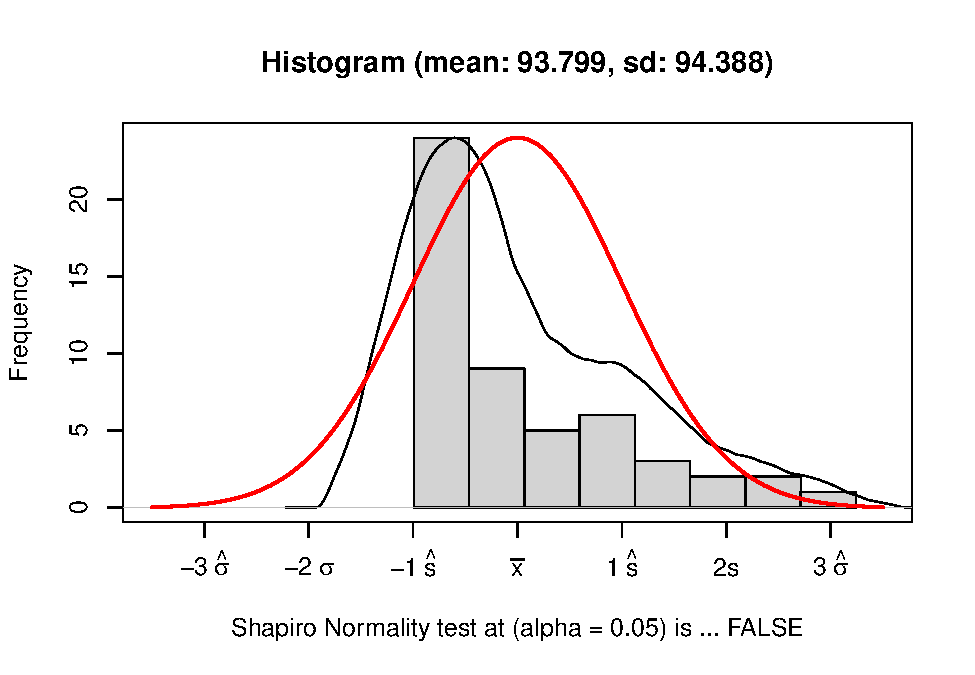
\includegraphics{Denzel-v-Will-data_files/figure-latex/unnamed-chunk-5-1.pdf}

\begin{Shaded}
\begin{Highlighting}[]
\KeywordTok{normalDiagnosticPlot}\NormalTok{(DGross)}
\end{Highlighting}
\end{Shaded}

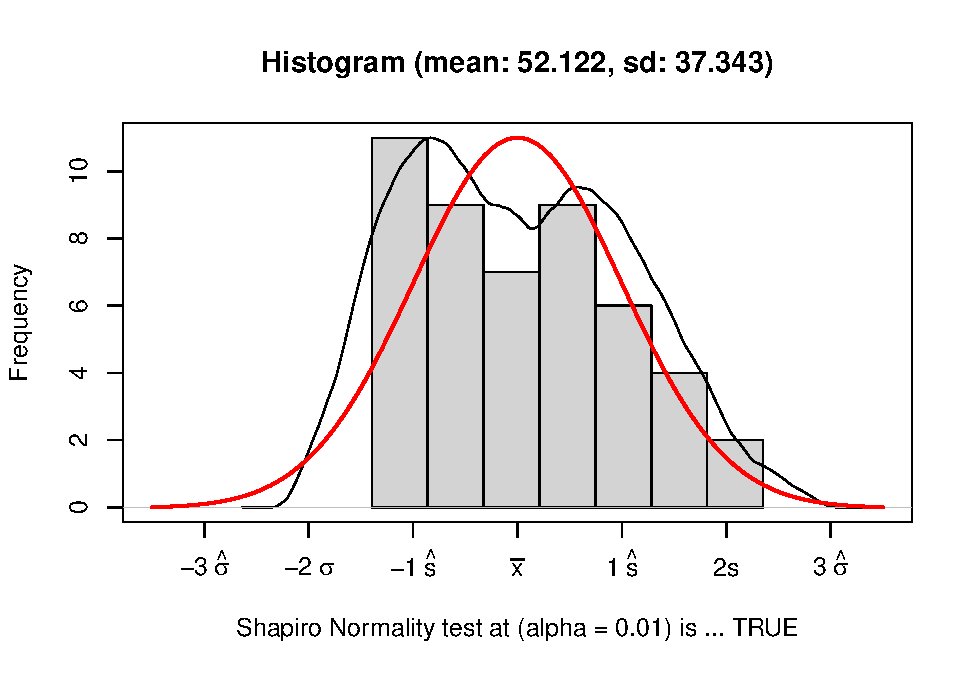
\includegraphics{Denzel-v-Will-data_files/figure-latex/unnamed-chunk-5-2.pdf}

\begin{Shaded}
\begin{Highlighting}[]
\KeywordTok{hist}\NormalTok{(WGross, }\DataTypeTok{main =} \StringTok{"Histogram of Will Smith movie Grosses"}\NormalTok{)}
\end{Highlighting}
\end{Shaded}

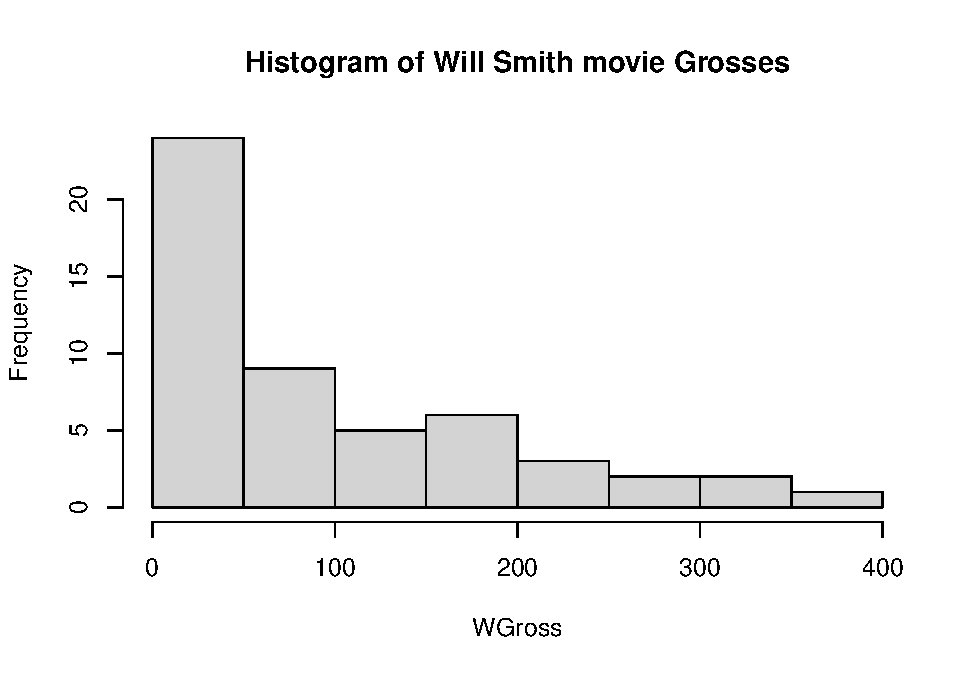
\includegraphics{Denzel-v-Will-data_files/figure-latex/unnamed-chunk-5-3.pdf}

\begin{Shaded}
\begin{Highlighting}[]
\KeywordTok{hist}\NormalTok{(DGross, }\DataTypeTok{main =} \StringTok{"Histogram of Denzels movie Grosses"}\NormalTok{)}
\end{Highlighting}
\end{Shaded}

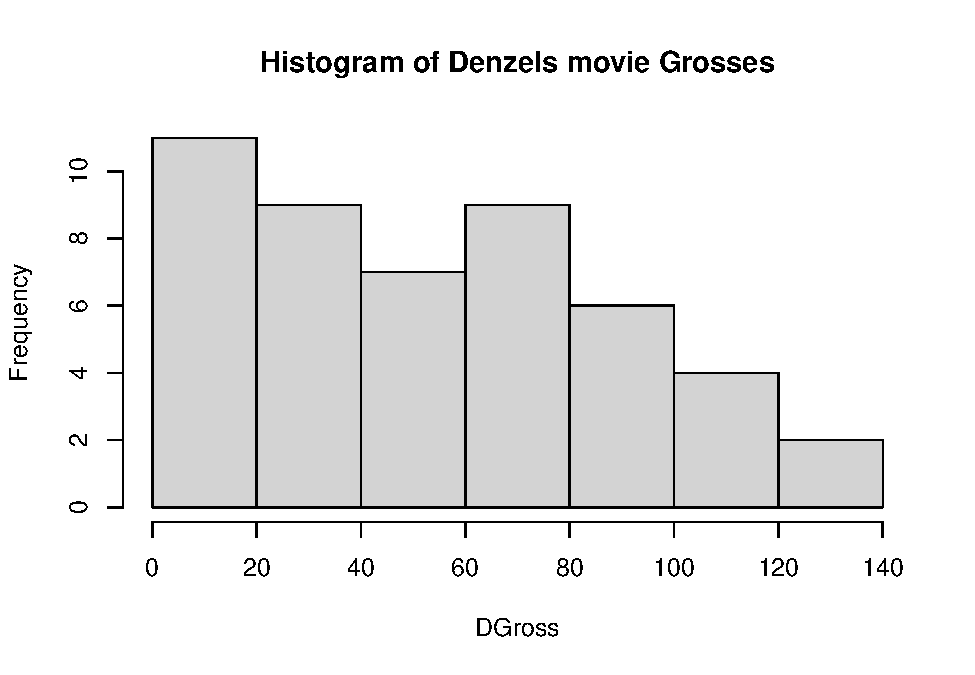
\includegraphics{Denzel-v-Will-data_files/figure-latex/unnamed-chunk-5-4.pdf}

\begin{Shaded}
\begin{Highlighting}[]
\KeywordTok{t.test}\NormalTok{(WGross, DGross)}
\end{Highlighting}
\end{Shaded}

\begin{verbatim}
## 
##  Welch Two Sample t-test
## 
## data:  WGross and DGross
## t = 2.9442, df = 67.651, p-value = 0.004434
## alternative hypothesis: true difference in means is not equal to 0
## 95 percent confidence interval:
##  13.42761 69.92714
## sample estimates:
## mean of x mean of y 
##  93.79904  52.12167
\end{verbatim}

\begin{Shaded}
\begin{Highlighting}[]
\NormalTok{Wyear =}\StringTok{ }\NormalTok{myWill.df}\OperatorTok{$}\NormalTok{year}
\NormalTok{Dyear =}\StringTok{ }\NormalTok{myDenzel.df}\OperatorTok{$}\NormalTok{year}

\KeywordTok{plot}\NormalTok{(WillRatings, Wyear)}
\NormalTok{reg.n =}\StringTok{ }\KeywordTok{lm}\NormalTok{(Wyear }\OperatorTok{\textasciitilde{}}\StringTok{ }\NormalTok{WillRatings)}
\KeywordTok{abline}\NormalTok{(reg.n)}

\KeywordTok{abline}\NormalTok{(reg.n)}
\end{Highlighting}
\end{Shaded}

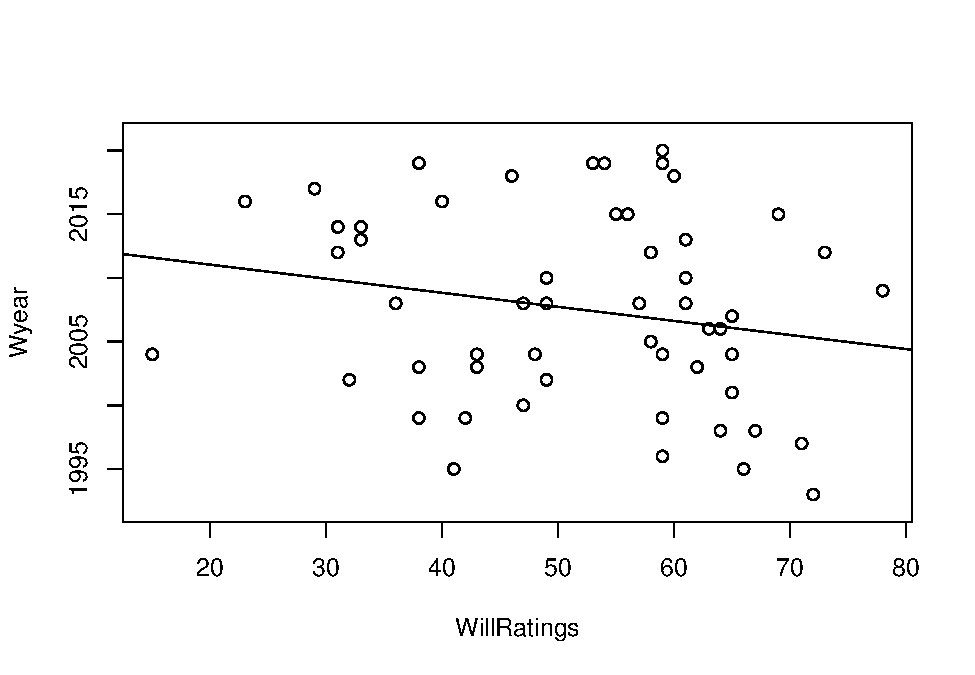
\includegraphics{Denzel-v-Will-data_files/figure-latex/unnamed-chunk-5-5.pdf}

\begin{Shaded}
\begin{Highlighting}[]
\NormalTok{plot1 =}\StringTok{ }\KeywordTok{plot}\NormalTok{(Dyear, DMovieRatings)}
\NormalTok{reg.n =}\StringTok{ }\KeywordTok{lm}\NormalTok{(DMovieRatings }\OperatorTok{\textasciitilde{}}\StringTok{ }\NormalTok{Dyear)}
\KeywordTok{abline}\NormalTok{(reg.n)}

\KeywordTok{abline}\NormalTok{(reg.n)}
\end{Highlighting}
\end{Shaded}

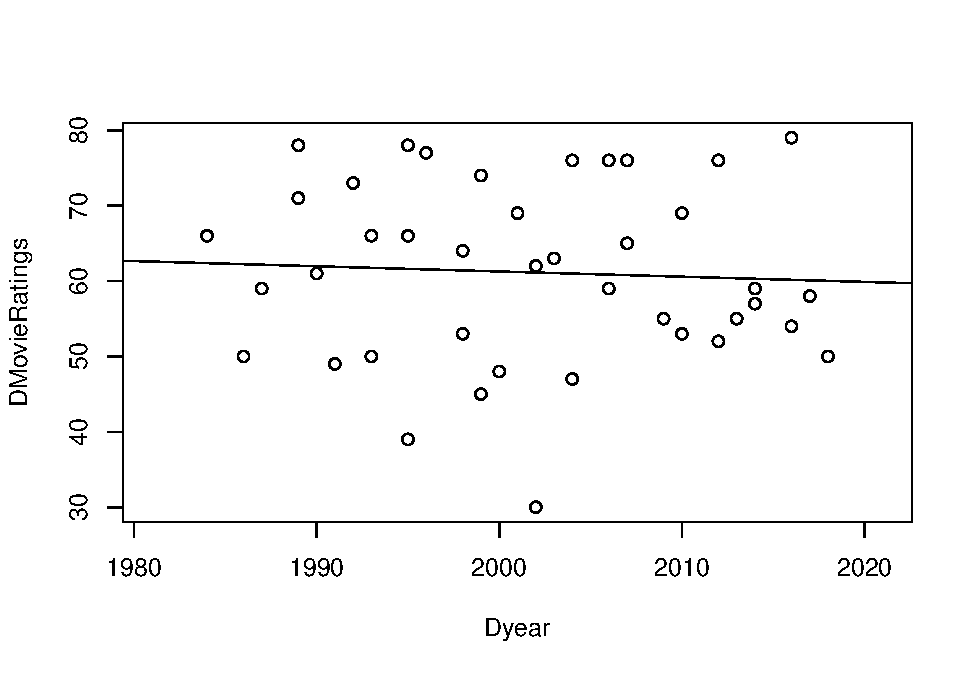
\includegraphics{Denzel-v-Will-data_files/figure-latex/unnamed-chunk-5-6.pdf}

\begin{Shaded}
\begin{Highlighting}[]
\NormalTok{plot2 =}\StringTok{ }\KeywordTok{plot}\NormalTok{(Wyear, WGross)}
\NormalTok{reg.n =}\StringTok{ }\KeywordTok{lm}\NormalTok{(WGross }\OperatorTok{\textasciitilde{}}\StringTok{ }\NormalTok{Wyear, }\DataTypeTok{col =} \StringTok{"red"}\NormalTok{)}
\end{Highlighting}
\end{Shaded}

\begin{verbatim}
## Warning: In lm.fit(x, y, offset = offset, singular.ok = singular.ok, ...) :
##  extra argument 'col' will be disregarded
\end{verbatim}

\begin{Shaded}
\begin{Highlighting}[]
\KeywordTok{abline}\NormalTok{(reg.n)}

\KeywordTok{abline}\NormalTok{(reg.n)}
\end{Highlighting}
\end{Shaded}

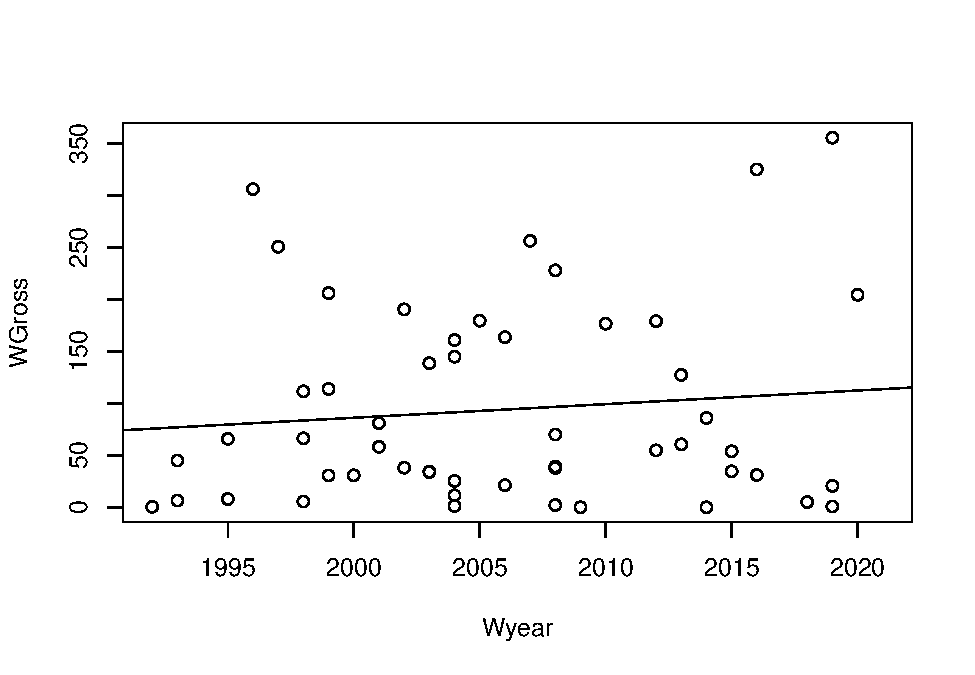
\includegraphics{Denzel-v-Will-data_files/figure-latex/unnamed-chunk-5-7.pdf}

\begin{Shaded}
\begin{Highlighting}[]
\KeywordTok{plot}\NormalTok{(Dyear, DGross)}
\NormalTok{reg.n =}\StringTok{ }\KeywordTok{lm}\NormalTok{(DGross }\OperatorTok{\textasciitilde{}}\StringTok{ }\NormalTok{Dyear)}
\KeywordTok{abline}\NormalTok{(reg.n)}

\KeywordTok{abline}\NormalTok{(reg.n)}
\end{Highlighting}
\end{Shaded}

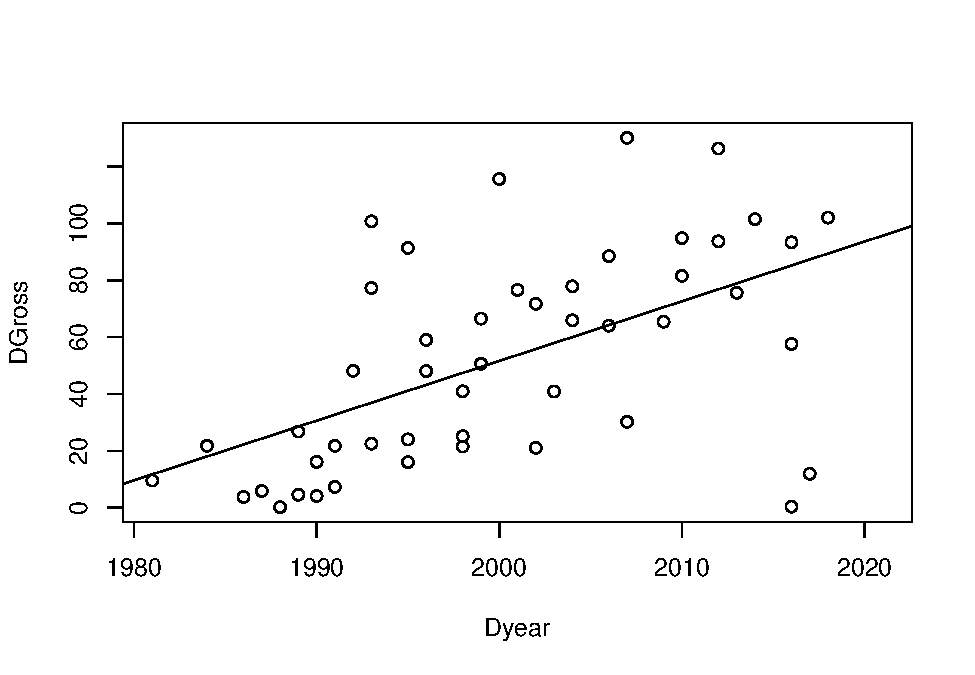
\includegraphics{Denzel-v-Will-data_files/figure-latex/unnamed-chunk-5-8.pdf}

\begin{Shaded}
\begin{Highlighting}[]
\KeywordTok{summary}\NormalTok{(will.movies)}
\end{Highlighting}
\end{Shaded}

\begin{verbatim}
##      ttid               nmid                rank            year     
##  Length:111         Length:111         Min.   :  1.0   Min.   :1992  
##  Class :character   Class :character   1st Qu.: 28.5   1st Qu.:2002  
##  Mode  :character   Mode  :character   Median : 56.0   Median :2007  
##                                        Mean   : 56.0   Mean   :2007  
##                                        3rd Qu.: 83.5   3rd Qu.:2014  
##                                        Max.   :111.0   Max.   :2021  
##                                                        NA's   :35    
##     title              genre              rated              minutes     
##  Length:111         Length:111         Length:111         Min.   : 52.0  
##  Class :character   Class :character   Class :character   1st Qu.: 93.5  
##  Mode  :character   Mode  :character   Mode  :character   Median :105.0  
##                                                           Mean   :106.3  
##                                                           3rd Qu.:118.0  
##                                                           Max.   :157.0  
##                                                           NA's   :40     
##     ratings        metacritic        votes           millions     
##  Min.   :2.300   Min.   :15.00   Min.   :    34   Min.   :  0.02  
##  1st Qu.:5.700   1st Qu.:41.50   1st Qu.: 11735   1st Qu.: 24.24  
##  Median :6.300   Median :56.00   Median : 56408   Median : 56.48  
##  Mean   :6.228   Mean   :51.98   Mean   :131488   Mean   : 93.80  
##  3rd Qu.:6.875   3rd Qu.:62.50   3rd Qu.:206926   3rd Qu.:161.54  
##  Max.   :8.600   Max.   :78.00   Max.   :675160   Max.   :355.56  
##  NA's   :37      NA's   :56      NA's   :45       NA's   :59      
##   paragraph        
##  Length:111        
##  Class :character  
##  Mode  :character  
##                    
##                    
##                    
## 
\end{verbatim}

\begin{Shaded}
\begin{Highlighting}[]
\KeywordTok{summary}\NormalTok{(denzel.movies)}
\end{Highlighting}
\end{Shaded}

\begin{verbatim}
##      ttid               nmid                rank         year     
##  Length:61          Length:61          Min.   : 1   Min.   :1981  
##  Class :character   Class :character   1st Qu.:16   1st Qu.:1994  
##  Mode  :character   Mode  :character   Median :31   Median :2001  
##                                        Mean   :31   Mean   :2002  
##                                        3rd Qu.:46   3rd Qu.:2011  
##                                        Max.   :61   Max.   :2021  
##                                                     NA's   :2     
##     title              genre              rated              minutes     
##  Length:61          Length:61          Length:61          Min.   : 60.0  
##  Class :character   Class :character   Class :character   1st Qu.:103.5  
##  Mode  :character   Mode  :character   Mode  :character   Median :118.0  
##                                                           Mean   :117.0  
##                                                           3rd Qu.:127.5  
##                                                           Max.   :202.0  
##                                                           NA's   :6      
##     ratings        metacritic        votes           millions     
##  Min.   :5.000   Min.   :30.00   Min.   :   330   Min.   :  0.19  
##  1st Qu.:6.500   1st Qu.:53.00   1st Qu.: 13118   1st Qu.: 21.43  
##  Median :6.850   Median :61.00   Median : 74561   Median : 49.42  
##  Mean   :6.815   Mean   :61.15   Mean   :113021   Mean   : 52.12  
##  3rd Qu.:7.300   3rd Qu.:71.00   3rd Qu.:183051   3rd Qu.: 78.82  
##  Max.   :8.500   Max.   :79.00   Max.   :383980   Max.   :130.16  
##  NA's   :7       NA's   :20      NA's   :11       NA's   :13      
##   paragraph        
##  Length:61         
##  Class :character  
##  Mode  :character  
##                    
##                    
##                    
## 
\end{verbatim}

Reviews

You can see that Denzels reviews are much more stable

\begin{Shaded}
\begin{Highlighting}[]
\NormalTok{willReviews =}\StringTok{ }\NormalTok{will.movies}

\NormalTok{Wreviews =}\StringTok{ }\NormalTok{willReviews}\OperatorTok{$}\NormalTok{ratings}

\NormalTok{DenzelReviews =}\StringTok{ }\NormalTok{denzel.movies}

\NormalTok{DReviews =}\StringTok{ }\NormalTok{DenzelReviews}\OperatorTok{$}\NormalTok{ratings}

\KeywordTok{plot}\NormalTok{(Wreviews, }\DataTypeTok{type =} \StringTok{"l"}\NormalTok{, }\DataTypeTok{lwd =} \DecValTok{2}\NormalTok{, }\DataTypeTok{col =} \StringTok{"red"}\NormalTok{)}
\end{Highlighting}
\end{Shaded}

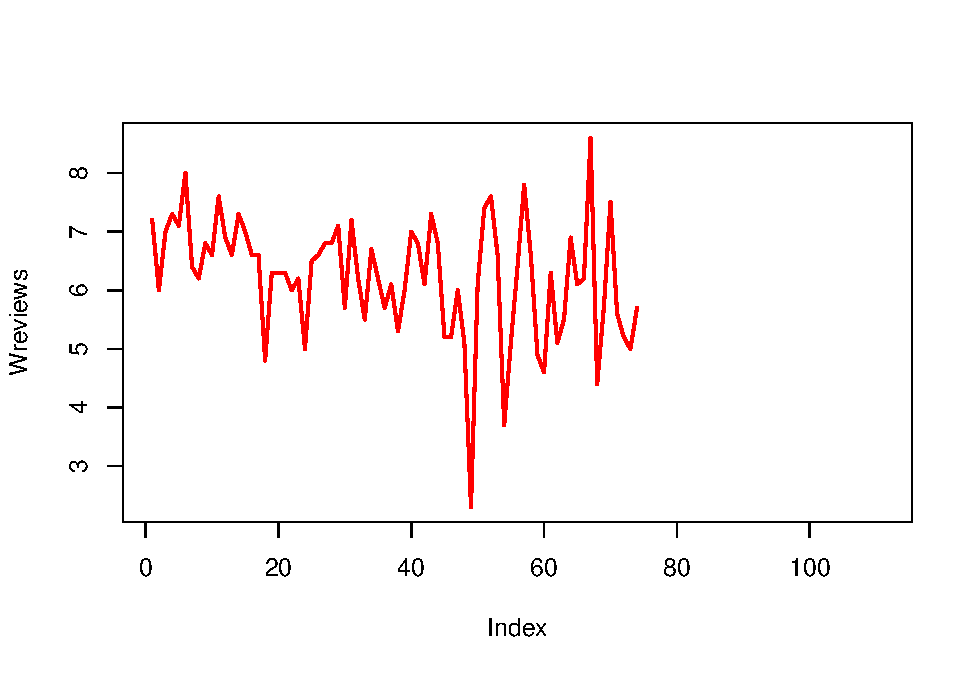
\includegraphics{Denzel-v-Will-data_files/figure-latex/unnamed-chunk-6-1.pdf}

\begin{Shaded}
\begin{Highlighting}[]
\KeywordTok{plot}\NormalTok{(DReviews, }\DataTypeTok{type =} \StringTok{"l"}\NormalTok{, }\DataTypeTok{lwd =} \DecValTok{2}\NormalTok{, }\DataTypeTok{col =} \StringTok{"red"}\NormalTok{)}
\end{Highlighting}
\end{Shaded}

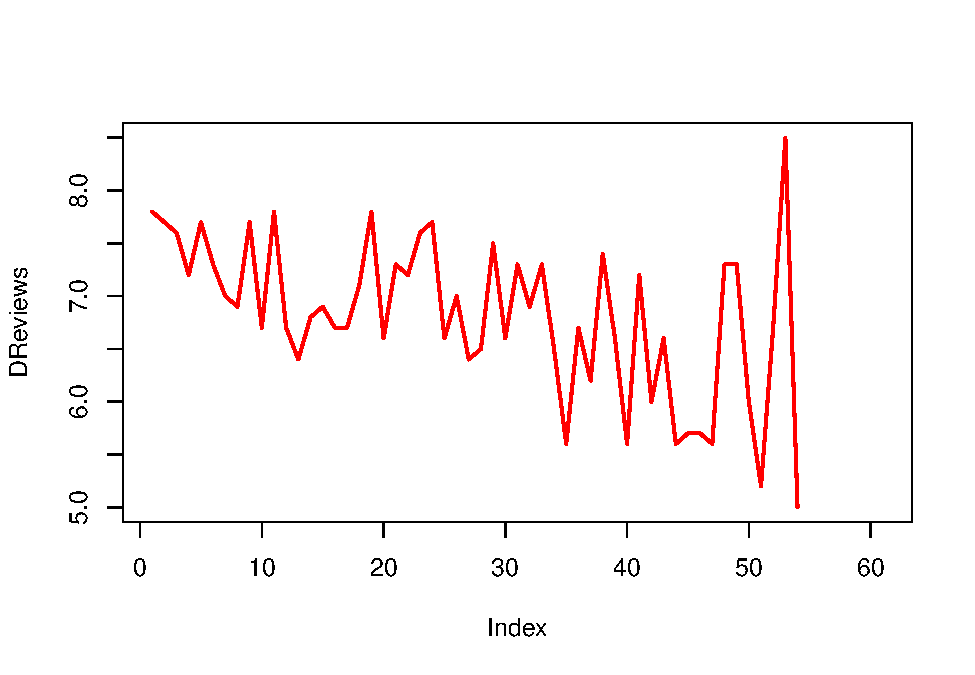
\includegraphics{Denzel-v-Will-data_files/figure-latex/unnamed-chunk-6-2.pdf}

\begin{Shaded}
\begin{Highlighting}[]
\KeywordTok{hist}\NormalTok{(Wreviews)}
\end{Highlighting}
\end{Shaded}

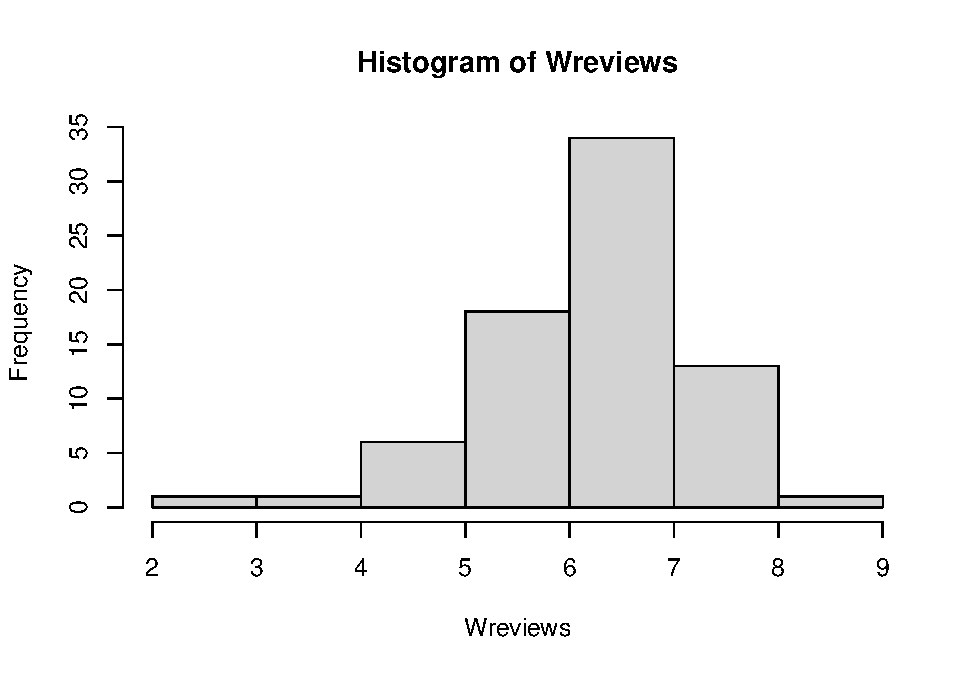
\includegraphics{Denzel-v-Will-data_files/figure-latex/unnamed-chunk-6-3.pdf}

\begin{Shaded}
\begin{Highlighting}[]
\KeywordTok{hist}\NormalTok{(DReviews)}
\end{Highlighting}
\end{Shaded}

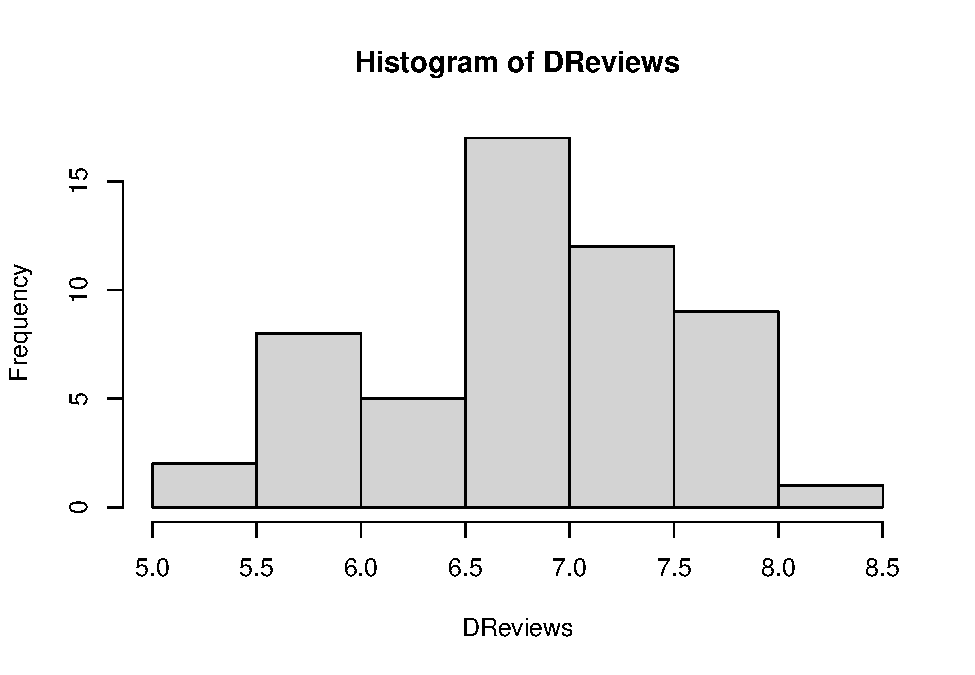
\includegraphics{Denzel-v-Will-data_files/figure-latex/unnamed-chunk-6-4.pdf}

\begin{Shaded}
\begin{Highlighting}[]
\KeywordTok{normalDiagnosticPlot}\NormalTok{(willReviews}\OperatorTok{$}\NormalTok{ratings)}
\end{Highlighting}
\end{Shaded}

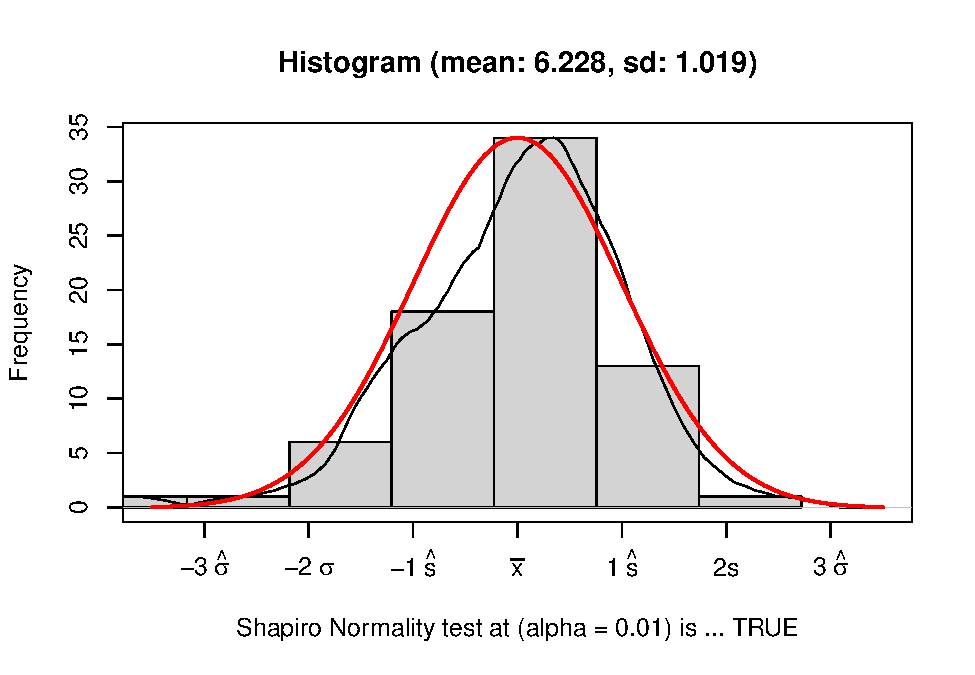
\includegraphics{Denzel-v-Will-data_files/figure-latex/unnamed-chunk-6-5.pdf}

\begin{Shaded}
\begin{Highlighting}[]
\KeywordTok{normalDiagnosticPlot}\NormalTok{(DenzelReviews}\OperatorTok{$}\NormalTok{ratings)}
\end{Highlighting}
\end{Shaded}

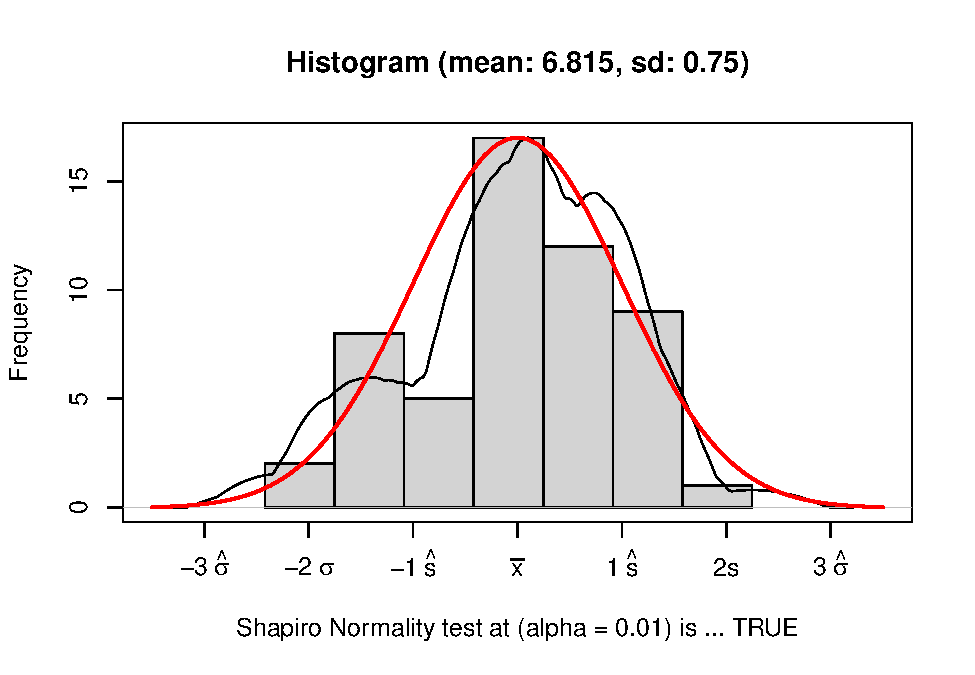
\includegraphics{Denzel-v-Will-data_files/figure-latex/unnamed-chunk-6-6.pdf}

\begin{Shaded}
\begin{Highlighting}[]
\KeywordTok{t.test}\NormalTok{(Wreviews, DReviews)}
\end{Highlighting}
\end{Shaded}

\begin{verbatim}
## 
##  Welch Two Sample t-test
## 
## data:  Wreviews and DReviews
## t = -3.7499, df = 125.99, p-value = 0.0002684
## alternative hypothesis: true difference in means is not equal to 0
## 95 percent confidence interval:
##  -0.8959184 -0.2769545
## sample estimates:
## mean of x mean of y 
##  6.228378  6.814815
\end{verbatim}

Popularity vs year of movie (when were they popular)

\subsubsection{Tables of Descriptive Statistics and Correlations}
\label{sec:correlation-tables}
\begin{table}[!htbp]
\footnotesize
\centering
\caption{\textbf{will smith correlation}}
\label{table:correlation}
\begin{tabularx}{0.95\textwidth}{{r@{ \ \ } p{35mm} r@{}lp{1mm} r@{}l p{5mm} r@{}l p{2mm} r@{}l p{2mm}   r@{}l  }}
 & \\
\hline
 & \\
\multicolumn{2}{c}{\textbf{ }} & \multicolumn{2}{c}{\textbf{M}} & & \multicolumn{2}{c}{\textbf{SD}} &  & \multicolumn{2}{c}{\textbf{1}} &  & \multicolumn{2}{c}{\textbf{2}} &  & \\ 
 & \\
\hline
 & \\
\textbf{1} & \textbf{metacritic} &  51&.4 &  &  14&.06 &  &  1&  &  &  \multicolumn{2}{c}{ \  \  \  \  \ }  &  & \\ 
 & \\
\textbf{2} & \textbf{millions} &  100&.5 &  &  95&.05 &  &  &.18 &  &  1&  &  & \\ 
 & \\
\textbf{3} & \textbf{year} &  2006&.3 &  &  7&.16 &  &  -&.30{$^{*}$}  &  &  &.08 &  & \\ 
 & \\
\hline
 & \\
\multicolumn{13}{p{0.86\textwidth}}{  \footnotesize { \begin{hangparas}{0.75in}{1} \textbf{\underline{Notes}:} \ \ Pearson pairwise correlations are reported; \newline a two-side test was performed to report correlation significance.  \end{hangparas} } }  & \\  
\multicolumn{13}{p{0.86\textwidth}}{  {\tiny {$^{\dagger} p < .10$} }  {     } {\tiny        {$^{*} p < .05$} }  {     } {\tiny       {$^{**} p < .01$} }  {     } {\tiny      {$^{***} p < .001$} } {     }     } & \\ 
 & \\
\hline
\end{tabularx}
\end{table}


\subsubsection{Tables of Descriptive Statistics and Correlations}
\label{sec:correlation-tables}
\begin{table}[!htbp]
\footnotesize
\centering
\caption{\textbf{Denzel Washington correlation}}
\label{table:correlation}
\begin{tabularx}{0.95\textwidth}{{r@{ \ \ } p{35mm} r@{}lp{1mm} r@{}l p{5mm} r@{}l p{2mm} r@{}l p{2mm}   r@{}l  }}
 & \\
\hline
 & \\
\multicolumn{2}{c}{\textbf{ }} & \multicolumn{2}{c}{\textbf{M}} & & \multicolumn{2}{c}{\textbf{SD}} &  & \multicolumn{2}{c}{\textbf{1}} &  & \multicolumn{2}{c}{\textbf{2}} &  & \\ 
 & \\
\hline
 & \\
\textbf{1} & \textbf{metacritic} &  51&.4 &  &  14&.06 &  &  1&  &  &  \multicolumn{2}{c}{ \  \  \  \  \ }  &  & \\ 
 & \\
\textbf{2} & \textbf{millions} &  100&.5 &  &  95&.05 &  &  &.18 &  &  1&  &  & \\ 
 & \\
\textbf{3} & \textbf{year} &  2006&.3 &  &  7&.16 &  &  -&.30{$^{*}$}  &  &  &.08 &  & \\ 
 & \\
\hline
 & \\
\multicolumn{13}{p{0.86\textwidth}}{  \footnotesize { \begin{hangparas}{0.75in}{1} \textbf{\underline{Notes}:} \ \ Pearson pairwise correlations are reported; \newline a two-side test was performed to report correlation significance.  \end{hangparas} } }  & \\  
\multicolumn{13}{p{0.86\textwidth}}{  {\tiny {$^{\dagger} p < .10$} }  {     } {\tiny        {$^{*} p < .05$} }  {     } {\tiny       {$^{**} p < .01$} }  {     } {\tiny      {$^{***} p < .001$} } {     }     } & \\ 
 & \\
\hline
\end{tabularx}
\end{table}


\begin{Shaded}
\begin{Highlighting}[]
\KeywordTok{library}\NormalTok{(gtsummary)}
\end{Highlighting}
\end{Shaded}

\begin{verbatim}
## Warning: package 'gtsummary' was built under R version 4.0.3
\end{verbatim}

\begin{Shaded}
\begin{Highlighting}[]
\KeywordTok{library}\NormalTok{(dplyr)}

\NormalTok{myWill.df =}\StringTok{ }\NormalTok{will.movies}

\NormalTok{WillYears=}\StringTok{ }\NormalTok{myWill.df}\OperatorTok{$}\NormalTok{year}

\NormalTok{myDenzel.df =}\StringTok{ }\NormalTok{denzel.movies}
\NormalTok{denzelyear =}\StringTok{ }\NormalTok{myDenzel.df}\OperatorTok{$}\NormalTok{year}

\NormalTok{WGross =}\StringTok{ }\NormalTok{myWill.df}\OperatorTok{$}\NormalTok{millions}
\NormalTok{DGross =}\StringTok{ }\NormalTok{myDenzel.df}\OperatorTok{$}\NormalTok{millions}

\KeywordTok{plot}\NormalTok{(WillYears, WGross)}
\NormalTok{reg.n =}\StringTok{ }\KeywordTok{lm}\NormalTok{(WGross }\OperatorTok{\textasciitilde{}}\StringTok{ }\NormalTok{WillYears)}
\KeywordTok{abline}\NormalTok{(reg.n)}

\KeywordTok{abline}\NormalTok{(reg.n)}
\end{Highlighting}
\end{Shaded}

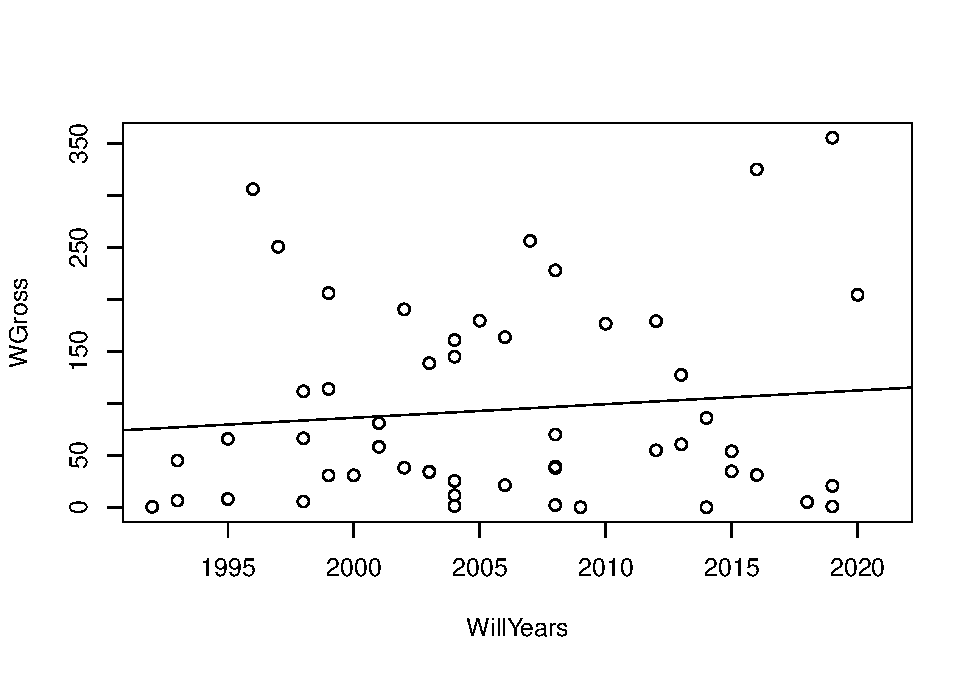
\includegraphics{Denzel-v-Will-data_files/figure-latex/unnamed-chunk-7-1.pdf}

\begin{Shaded}
\begin{Highlighting}[]
\KeywordTok{plot}\NormalTok{(denzelyear, DGross)}
\NormalTok{reg.n =}\StringTok{ }\KeywordTok{lm}\NormalTok{(DGross }\OperatorTok{\textasciitilde{}}\StringTok{ }\NormalTok{denzelyear)}
\KeywordTok{abline}\NormalTok{(reg.n)}

\KeywordTok{abline}\NormalTok{(reg.n)}
\end{Highlighting}
\end{Shaded}

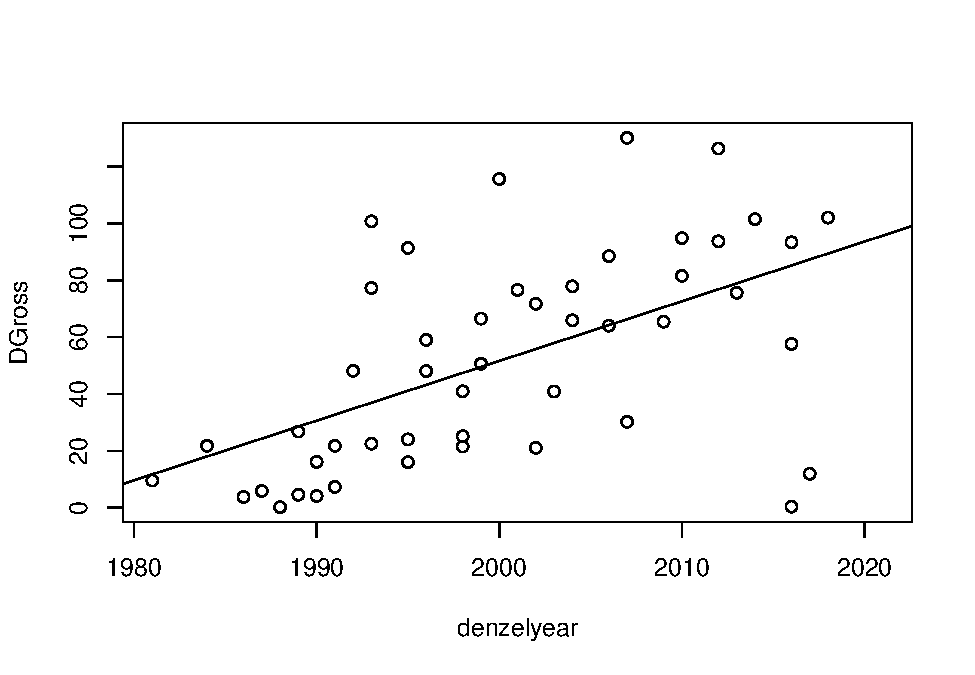
\includegraphics{Denzel-v-Will-data_files/figure-latex/unnamed-chunk-7-2.pdf}

\begin{Shaded}
\begin{Highlighting}[]
\KeywordTok{hist}\NormalTok{(WillYears)}
\end{Highlighting}
\end{Shaded}

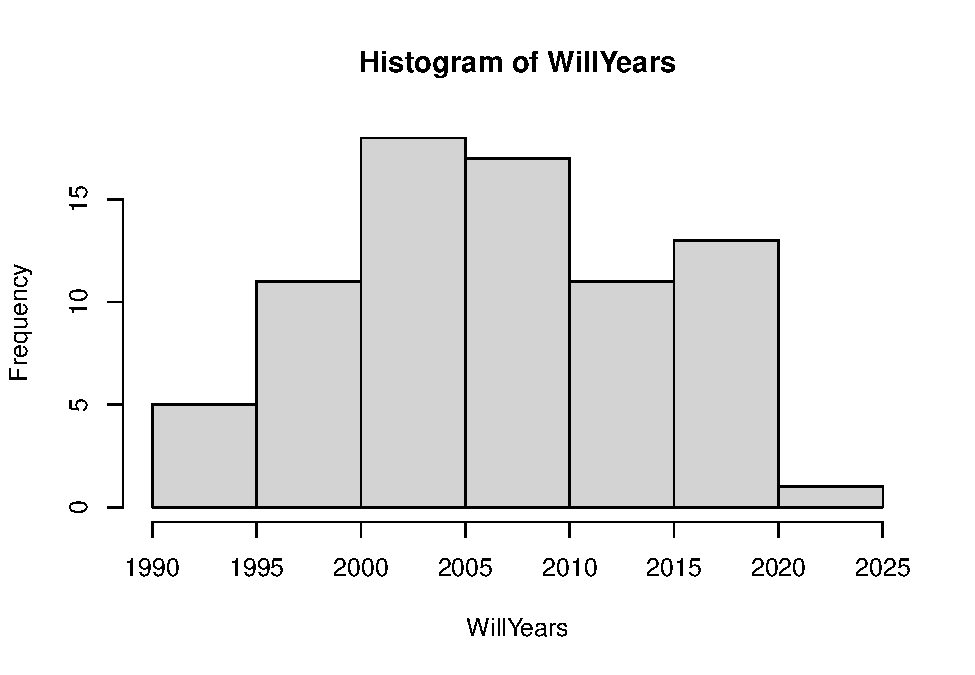
\includegraphics{Denzel-v-Will-data_files/figure-latex/unnamed-chunk-7-3.pdf}

\begin{Shaded}
\begin{Highlighting}[]
\KeywordTok{hist}\NormalTok{(denzelyear)}
\end{Highlighting}
\end{Shaded}

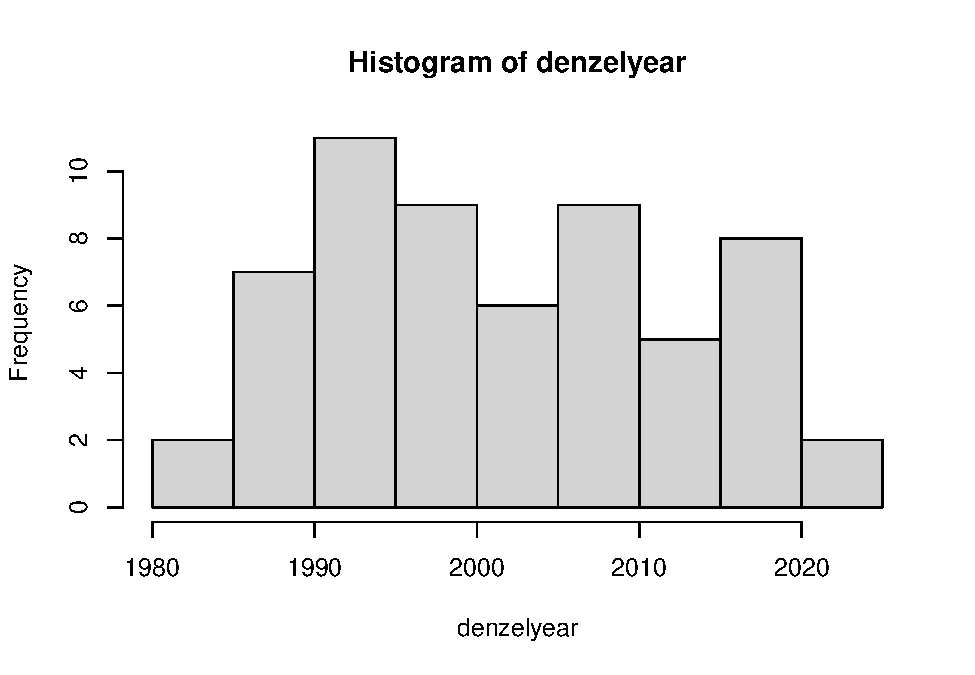
\includegraphics{Denzel-v-Will-data_files/figure-latex/unnamed-chunk-7-4.pdf}

\begin{Shaded}
\begin{Highlighting}[]
\NormalTok{total \textless{}{-}}\StringTok{ }\KeywordTok{merge}\NormalTok{(myWill.df, myDenzel.df, }\DataTypeTok{by=}\StringTok{"year"}\NormalTok{)}
\CommentTok{\#total}

\KeywordTok{t.test}\NormalTok{(WGross, DGross)}
\end{Highlighting}
\end{Shaded}

\begin{verbatim}
## 
##  Welch Two Sample t-test
## 
## data:  WGross and DGross
## t = 2.9442, df = 67.651, p-value = 0.004434
## alternative hypothesis: true difference in means is not equal to 0
## 95 percent confidence interval:
##  13.42761 69.92714
## sample estimates:
## mean of x mean of y 
##  93.79904  52.12167
\end{verbatim}

\begin{Shaded}
\begin{Highlighting}[]
\CommentTok{\#zero = myWill.df[,c("rating","millions")]}
\KeywordTok{summary}\NormalTok{(myWill.df)}
\end{Highlighting}
\end{Shaded}

\begin{verbatim}
##      ttid               nmid                rank            year     
##  Length:111         Length:111         Min.   :  1.0   Min.   :1992  
##  Class :character   Class :character   1st Qu.: 28.5   1st Qu.:2002  
##  Mode  :character   Mode  :character   Median : 56.0   Median :2007  
##                                        Mean   : 56.0   Mean   :2007  
##                                        3rd Qu.: 83.5   3rd Qu.:2014  
##                                        Max.   :111.0   Max.   :2021  
##                                                        NA's   :35    
##     title              genre              rated              minutes     
##  Length:111         Length:111         Length:111         Min.   : 52.0  
##  Class :character   Class :character   Class :character   1st Qu.: 93.5  
##  Mode  :character   Mode  :character   Mode  :character   Median :105.0  
##                                                           Mean   :106.3  
##                                                           3rd Qu.:118.0  
##                                                           Max.   :157.0  
##                                                           NA's   :40     
##     ratings        metacritic        votes           millions     
##  Min.   :2.300   Min.   :15.00   Min.   :    34   Min.   :  0.02  
##  1st Qu.:5.700   1st Qu.:41.50   1st Qu.: 11735   1st Qu.: 24.24  
##  Median :6.300   Median :56.00   Median : 56408   Median : 56.48  
##  Mean   :6.228   Mean   :51.98   Mean   :131488   Mean   : 93.80  
##  3rd Qu.:6.875   3rd Qu.:62.50   3rd Qu.:206926   3rd Qu.:161.54  
##  Max.   :8.600   Max.   :78.00   Max.   :675160   Max.   :355.56  
##  NA's   :37      NA's   :56      NA's   :45       NA's   :59      
##   paragraph        
##  Length:111        
##  Class :character  
##  Mode  :character  
##                    
##                    
##                    
## 
\end{verbatim}




%% appendices go here!


\newpage
\theendnotes

%%%%%%%%%%%%%%%%%%%%%%%%%%%%%%%%%%%  biblio %%%%%%%%
\newpage
\begin{auxmulticols}{2}
\singlespacing 
\bibliography{./../biblio/master.bib}

%%%%%%%%%%%%%%%%%%%%%%%%%%%%%%%%%%%  biblio %%%%%%%%
\end{auxmulticols}

\newpage
{
\hypersetup{linkcolor=black}
\setcounter{tocdepth}{3}
\tableofcontents
}



\end{document}